\subsection{Influencia de $k_{ij}$ sobre $f$}

Sin importar la estrategia de forrajeo tenemos que :
\begin{enumerate}[label=(\alph*)]
\item \begin{equation}
  \lim_{k_{ij} \to  0 }f(k_{ij}) = \lim_{k_{ij} \to 0 }\frac{g(k_{ij}) a}{1+k_{ij}^\phi} = 0 
\end{equation}
ya que $ g(k_{ij}) \to (k_{ij} \to 0)$ y $\frac{a}{1+k_{ij}^\phi} < a$  para todo $k_{ij}$
\item 
\begin{equation}
\lim_{k_{ij} \to  0 }f(k_{ij}) - ag(k_{ij}) = 0
\end{equation}
y por lo tanto $f \approx a g(k_{ij})$ para $k_{ij}$ suficientemente peque\~no , donde $g(k_{ij}) = f(k_{ij})\Pi(k_{ij})$.
\item $f_{3D} > f_{2D} \iff k_{ij} > 1$ donde $f_{nD}$ representa al valor de $f$ para espacios de b\'usqueda \emph{n-dimensionales}
\end{enumerate}

A continuaci\'on se analizan propiedades de $f$ que a nivel \emph{cuantitativo} difieren entre las distintas estrategias de forrajeo

\subsubsection{Grazing}

\begin{prop}
  $f$ tiene un punto m\'aximo en $\mathbb{R}^+$ si y solo s\'i $\phi > (D_i - 1)p_d$ 
\end{prop}

\begin{proof}
\mbox{}\\
Sea $ h = (D_i-1)p_d$\\
Dado que $f$ es diferenciable y:
  \begin{equation}
    \begin{aligned}
      f'(k_{ij}) &= a \frac{h k_{ij}^{h-1} (1 + k_{ij}^\phi) -\phi k_{ij}^{\phi-1+h}}{(1+k_{ij}^{\phi})^2} \\
            &= a \frac{(h-\phi)k_{ij}^{h-1 + \phi}  + h k_{ij}^{h-1} }{(1+k_{ij}^{\phi})^2}\\
            &= a \frac{(h-\phi)k_{ij}^\phi + h }{(1+k_{ij}^{\phi})^2}\\
     \end{aligned}
  \end{equation}
Luego tenemos que $f'$ posee un \emph{cero} en $\mathbb{R}^+$ si y solo s\'i $ h< \phi$ y en caso afirmativo tenemos que $k^*$ tal que $f(k^*) = 0$ es $(\frac{h}{\phi-h})^{\frac{1}{\phi}}$ adem\'as:
\begin{equation}
  f'(x) :
  \begin{cases}
    < 0 &; k_{ij}  > k^* \\
    > 0 &; k_{ji} < k^*
  \end{cases}
\end{equation}

Lo que indica que $k^*$ es un punto m\'aximo.
\end{proof}

De la proposici\'on anterior tambi\'en vemos la dependencia de $k^*$ en $\phi$, teniendo $h$ fijo en nuestro caso se observa que si $\phi$ esta suficientemente cercano a $h$ , $k^*$ es extremadamente grande, sin embargo se observa un decaim\'iento muy r\'apido y para valores de $\phi \geq 2h$  , $k^*$ se encuentra pr\'oximo a 1(y en realidad converge a 1 para $\phi \to \infty$) , v\'ease figura \ref{fig:kmaxGrazing}. \\

\begin{figure}
\begin{center}
 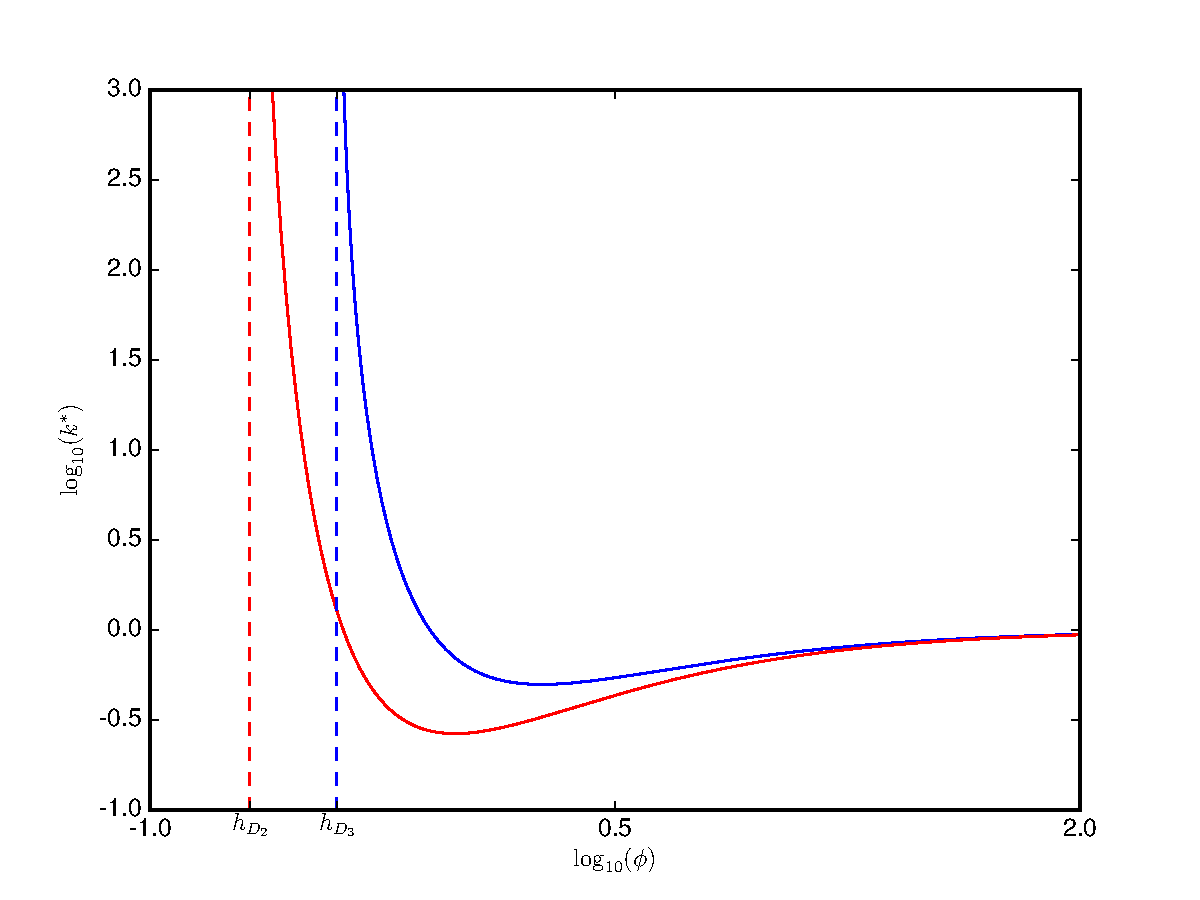
\includegraphics[width=0.9\textwidth]{./Plots/kmaxGrazing.pdf}
 \caption[$k^*, Grazing$]{$k^*$ en funci\'on a $\phi$ donde se observa la divergencia para valores cercanos a $h$ y la convergencia a 1 para valores elevados de $\phi$, ({\hwplotB}) es para el caso de ambientes de b\'usqueda $3D$ y ({\hwplotR}) $2D$, $h_{3D}$ y $h_{2D}$ denotan los l\'imites inferiores para $\phi$ que permiten la existencia de $k^*$}
 \label{fig:kmaxGrazing} 
\end{center}
\end{figure}



En el caso que $\phi < h$ tenemos que $f$ es mon\'otona creciente. Ambos casos se grafican en la figura \ref{fig:f1Grazing}.

\begin{figure}
\begin{center}
 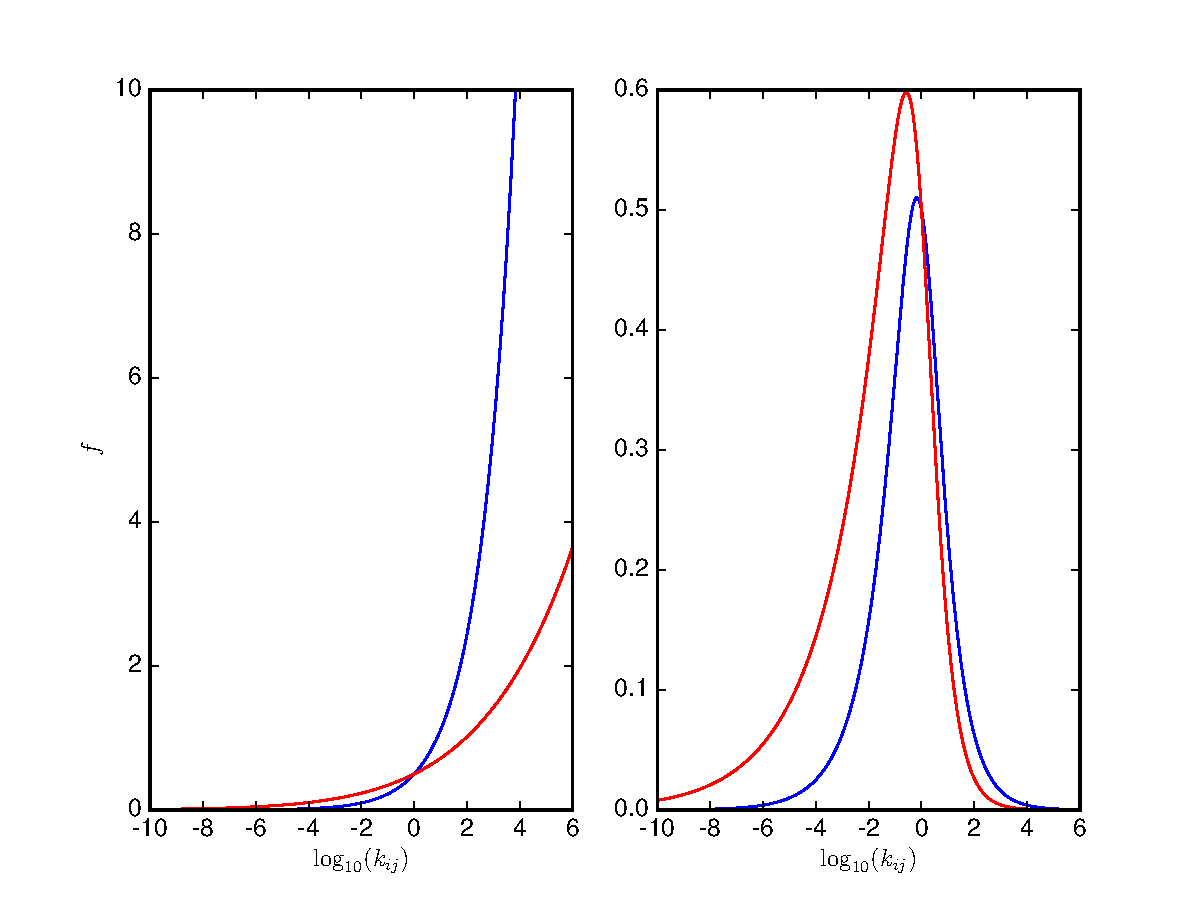
\includegraphics[width=0.9\textwidth]{./Plots/f1Grazing.pdf}
 \caption[$f_1, Grazing$]{$f$ en funci\'on a $k_{ij}$, con $a =1$, en el panel de la izquierda tenemos $b = 0.1$ y en el de la derecha $b=1.$ , ({\hwplotB}) es para el caso de ambientes de b\'usqueda $3D$ y ({\hwplotR}) $2D$}
 \label{fig:f1Grazing} 
\end{center}
\end{figure}


\subsubsection{Sit}

Se tiene cualitativamente las m\'ismas caracter\'isticas que en el caso anterior, con la diferencia que en este caso $ h:= p_v + 2(D_i -1) p_d$, y por ende para $\phi \in ]2(D_i - 1) p_d , p_V + 2(D_i -1)p_d[$ tendr\'iamos un comportamiento mon\'ontono para $f_{sit}$ y la existencia de un m\'aximo para $f_{grazing}$.\\

La figura \ref{fig:f1Sit} muestra las semejanzas con el caso anterior, salvo la diferencia que en este caso $k^*>1$ para el caso $3D$ y adem\'as alcanza un valor m\'as alto que el caso $2D$.\\
En general tenemos que $ k^*_{Sit} > k^*_{grazing}$ .

\begin{figure}
\begin{center}
 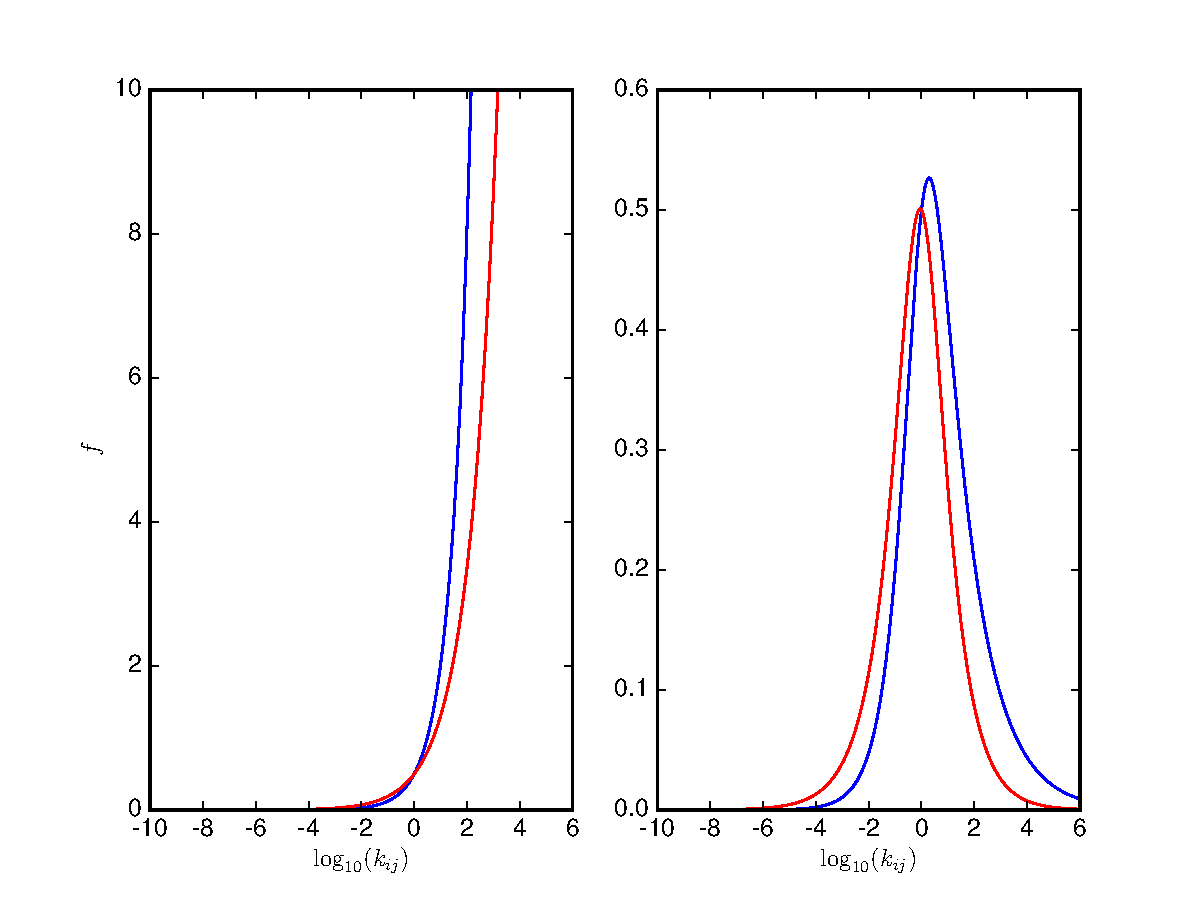
\includegraphics[width=0.9\textwidth]{./Plots/f1Sit.pdf}
 \caption[$f_1, Sit$]{$f$ en funci\'on a $k_{ij}$, con $a =1$, para el caso de una estrategia de forrajeo \emph{Sit-and-Wait}, las dem\'as especificaciones se comparten con la figura \ref{fig:f1Grazing}}
 \label{fig:f1Sit} 
\end{center}
\end{figure}


\subsubsection{Captura activa}

En este caso tenemos un comportamiento similar al descrito previamente, esto es para $\phi > p_v + 2(D_i -1) p_d$ tenemos que $f$ decae exponencialmente a partir de un valor de $k_{ij}$ \emph{suficientemente grande}, y a su vez crece exponencialmente para valores \emph{suficientemente peque\~nos}, dado que $f \in C^1$ esto a su vez nos dice que debe existir un punto m\'aximo para $f$ sin embargo en este caso no tenemos una expresi\'on an\'alitica para $k^*$ salvo que cumple la siguiente relaci\'on:

\begin{equation}
  (k^*)^{\phi}((k^*)^{2p_v}(p_v+ h -\phi) + (h -\phi) + (k^*)^{2p_v - \phi}(p_v + h ) ) + h = 0
\end{equation}

Con $h$ igual que en el caso $grazing$.\\
De esta relaci\'on podemos obtener que :
\begin{equation}
  k^*_{Active} \in ] k^*_{Grazing} , k^*_{Sit} [
\end{equation}

A su vez para $\phi \leq 2(D_i - 1)p_d $ podemos esperar un crecimiento mon\'otono por parte de $f$. 

\begin{figure}
\begin{center}
 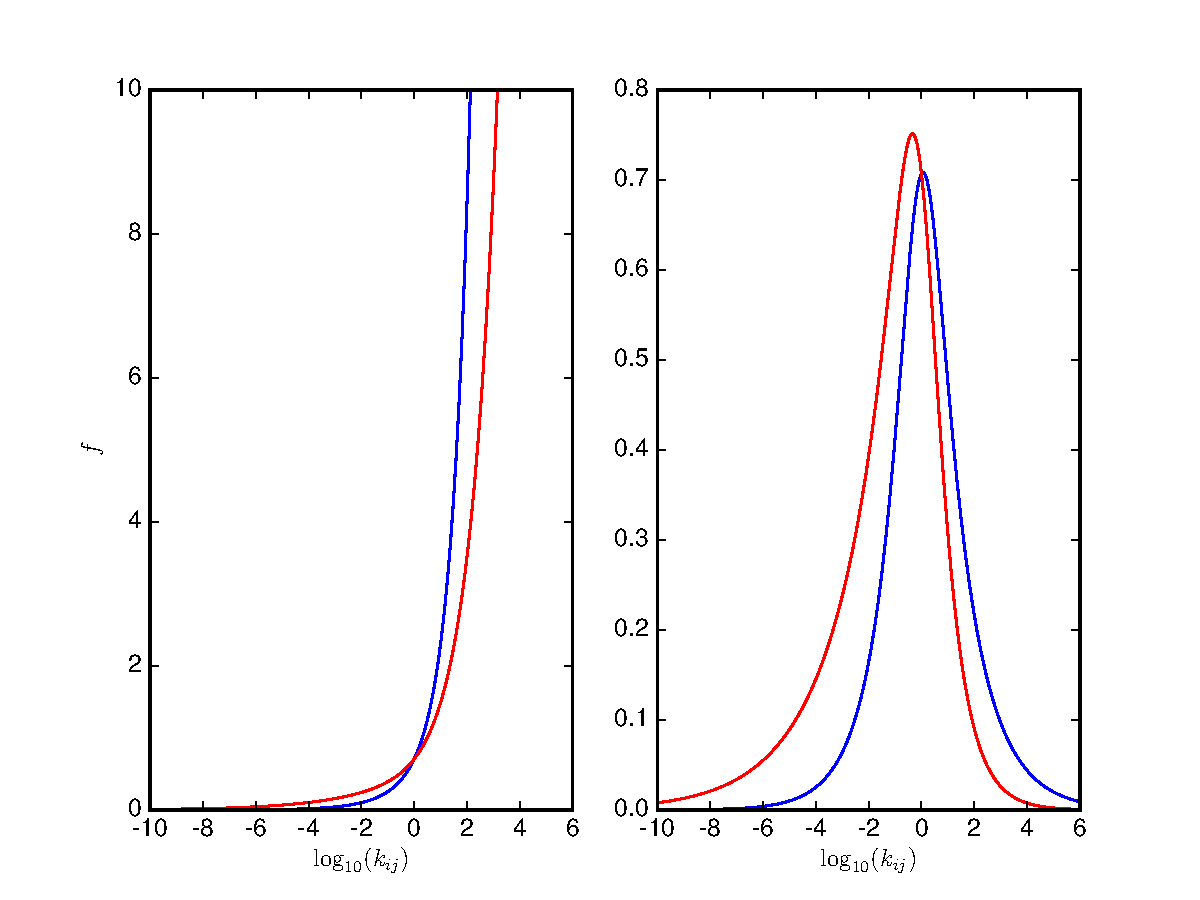
\includegraphics[width=0.9\textwidth]{./Plots/f1Active.pdf}
 \caption[$f_1, Active$]{$f$ en funci\'on a $k_{ij}$, con $a =1$, para el caso de una estrategia de forrajeo \emph{activa}, las dem\'as especificaciones se comparten con la figura \ref{fig:f1Grazing}}
 \label{fig:f1Active} 
\end{center}
\end{figure}




\subsection{Derivaci\'on de Criterios y Zonas de Invasibilidad}\label{subsec:CI}

En lo sucesivo $\mathbf{A}$ denota toda la zona par\'ametrica explorada,en nuestro caso 
\begin{enumerate}
\item $\mathbf{A} = [-14,6] \times [-10,5]$ , $k_{\CP} = k_{\RC}$
\item $\mathbf{A} = [-10,5] \times [-10,5]$ , $k_{\CP} \not= k_{\RC}$
\end{enumerate}

\subsubsection{R}
El sistema se reduce a:
\begin{equation}
\dot{R}= rR(1-R/K)
\end{equation}

Por lo tanto el criterio de invasibilidad para R , $\mathbf{IC_\R}$ es:

\begin{equation}\label{eq:ICR}
\mathbf{IC_\R} := \dot{R} > 0 \iff r > 0
\end{equation}

\begin{equation}
\mathbf{Z(I_{\R})} := \{ v \in \mathbf{A} / \dot{R}(v)>0 \}
\end{equation}

\subsubsection{C $\to$ R}
El sistema se reduce a :
\begin{equation}
\begin{aligned}
\dot{R} &= R\left[r(1-R/K)- (\alpha_{1}/m_C) C \right] \\
\dot{C} &= C \left[\epsilon_1 (\alpha_{1}/m_C) R  -q_1 \right]
\end{aligned}
\end{equation}


\begin{equation} \mathbf{IC_{\C \to \R}} := \dot{C} >0 \iff \epsilon_1(\alpha_1/m_C)\hat{R}_1 > q_1  \end{equation}
Donde $\hat{R}_1 = K$ entonces:
\begin{equation} \mathbf{IC_{\C \to \R}} := \epsilon_1(\alpha_1/m_C) K > q_1 \end{equation}
            
\begin{equation}
\mathbf{Z(I_{\C \to \R})} := \{v \in Z(I_{\R}) / \dot{C}(v) > 0\}
\end{equation}


\subsubsection{P $\to$ R}
El sistema es similar al caso anterior, intercambiando $P$ por $C$.

\begin{equation} \mathbf{IC_{\PP \to \R}} := \dot{P}>0 \iff \epsilon_2(\alpha_2/m_P) K > q_2 \end{equation}

\begin{equation}
\mathbf{Z(I_{\PP \to \R})} := \{v \in Z(I_{\R}) / \dot{P}(v) > 0\}
\end{equation}

            
\subsubsection{P $\to$ C-R}

\begin{equation} \mathbf{IC_{\PP \to \C-\R}} := \dot{P} >0 \iff \epsilon_2\alpha_2\hat{R}_2 + \epsilon_3\alpha_3\hat{C}_2 > q_2 m_P \end{equation}

Donde:
\begin{equation}
\begin{aligned}
\hat{R}_2 &= \frac{q_1 m_C}{\epsilon_1 \alpha_1} \\
\hat{C}_2 &=  r(\frac{m_C}{\alpha_1}) \left[ 1 - \frac{q_1 m_C}{\epsilon_1 \alpha_1 K} \right] 
\end{aligned}
\end{equation}

\begin{equation}
\mathbf{Z(I_{\PP \to \C-\R})} := \{v \in Z(I_{\C \to \R}) / \dot{P}(v) > 0\}
\end{equation}


\subsubsection{C $\to$ P-R}

\begin{equation} \mathbf{IC_{\C \to \PP-\R}} := \dot{C}>0 \iff \epsilon_1(\alpha_1/m_C)\hat{R} - (\alpha_3/m_P)\hat{P}> q_1 \end{equation}
Donde:
\begin{equation}
\begin{aligned}
\hat{R} & = \frac{q_2 m_P}{\epsilon_2 \alpha_2} \\
\hat{P} & = r(\frac{m_P}{\alpha_2}) \left[ 1- \frac{q_2 m_P}{\epsilon_2 \alpha_2 K} \right]
\end{aligned}
\end{equation}

\begin{equation}
\mathbf{Z(I_{\C \to \PP-\R})} := \{v \in Z(I_{\PP \to \R}) / \dot{C}(v) > 0\}
\end{equation}


El c\'alculo expl\'icito de los bordes de cada zona, se reduce a calcular los zeros de las funciones asociadas a ellos; para llevar a cabo esto se uso el algoritmo de optimizaci\'on brentq el cual esta incorporado en el paquete SciPy de Python.

\subsection{C\'alculo Expl\'icito de zonas de invasibilidad}

En esta secci\'on derivamos los criterios de invasibilidad en funci\'on de la raz\'on de masas ($k_{\RC},k_{\CP}$ y $k_{\RP}$) y la masa del depredador tope $m_P$, asumiendo que:
\begin{enumerate}
\item $D_R = D_C = D$
\item $\beta_R = \beta_C = \beta_P = \beta$
\end{enumerate}


\subsubsection{C $\to$ R}

\begin{equation}
  \frac{dC}{dt} >0 \iff  m_P > \zeta_1(k_{\RC},k_{\CP}) = (\frac{\chi_1}{\chi_0})^{\frac{1}{h_R +1 - 2\beta }}
\end{equation}
Donde:
\begin{equation}
  \begin{aligned}
    h_R &= p_v + 2(D_R - 1)p_d \\
    \chi_0 &= \varepsilon_1 \kappa_0\alpha_{0,1} f_1(k_{\RC})k_{\CP}^{h_R -1} k_{\RP}^{1-\beta} \\
    \chi_1 &= q_{0,1} k_{\CP}^{\beta-1} 
  \end{aligned}
\end{equation}
Entonces:
\begin{equation}
\mathbf{Z(I_{\C\to \R})} := \{ (k_{\RC},k_{\CP},m_P) \in \mathbb{R}^3_+ / m_p > \zeta_1(k_{\RC},k_{\CP}) \}
\end{equation}

\subsubsection{P $\to$ R}

\begin{equation}
  \frac{dP}{dt} >0 \iff  m_P > \zeta_2(k_{\RC},k_{\CP}) = (\frac{q_{0,2}}{\eta_0})^{\frac{1}{h_R +1 - 2\beta}}
\end{equation}
Donde:
\begin{equation}
  \begin{aligned}
    \eta_0 &= \varepsilon_2 \kappa_0\alpha_{0,2} f_2(k_{\RP})k_{\RP}^{1-\beta} \\
  \end{aligned}
\end{equation}


\begin{equation}
\mathbf{Z(I_{\PP \to \R})} := \{ (k_{\RC},k_{\CP},m_P) \in \mathbb{R}^3_+ / m_p > \zeta_2(k_{\RC},k_{\CP}) \}
\end{equation}


Definamos:
\begin{equation}
  h = p_v + 2(D-1)p_d
\end{equation}

\subsubsection{P $\to$ C-R}
\begin{equation}
  \frac{dP}{dt}  >0 \iff m_P > \zeta_3(k_{\RC},k_{\CP}) = (\frac{\xi_4\xi_2}{\xi_3 + \xi_4 - q_{0,2}})^{\frac{1}{h + 1 - 2\beta}}
\end{equation}

Donde:
\begin{equation}
  \begin{aligned}
    \xi_0 &= \frac{q_{0,1} k_{\CP}^{\beta - h}}{\epsilon_1 \alpha_{0,1} f_1(k_{\RC})}\\
    \xi_1 &= \frac{r_0 k_{\RP}^{\beta -1}}{\alpha_{0,1} f_1(k_{\RC}) k_{\CP}^{h - 1}}\\
    \xi_2 &= \frac{\xi_0}{k_0 k_{\RP}^{1-\beta}} \\
    \xi_3 &= \epsilon_2 \alpha_{0,2} f_2(k_{\RP}) \xi_0\\
    \xi_4 &=\epsilon_3 \alpha_{0,3} f_3(k_{\CP}) \xi_1
  \end{aligned}
\end{equation}


Por lo tanto 
\begin{equation}
\mathbf{Z(I_{\PP \to \C-\R})} := \{ (k_{\RC},k_{\CP},m_P) \in \mathbb{R}^3_+ / m_p > \max\{\zeta_1(k_{\RC},k_{\CP}),\zeta_3(k_{\RC},k_{\CP})\} \}
\end{equation}
\subsubsection{C $\to$ P-R}
\begin{equation}
  \frac{dC}{dt}  >0 \iff m_P < \zeta_4(k_{\RC},k_{\CP}) = (\frac{\gamma_4\gamma_2}{\gamma_5 + \gamma_4 - \gamma_3})^{\frac{1}{h + 1 - 2\beta}}
\end{equation}

Donde:
\begin{equation}
  \begin{aligned}
    \gamma_0 &= \frac{q_{0,2}}{\varepsilon_2 \alpha_{0,2} f_2(k_{\RP})}\\
    \gamma_1 &= \frac{r_0 k_{\RP}^{\beta -1}}{\alpha_{0,2} f_2(k_{\RC})}\\
    \gamma_2 &= \frac{\gamma_0}{k_0 k_{\RP}^{1-\beta}} \\
    \gamma_3 &= \varepsilon_1\alpha_{0,1} f_1(k_{\RP}) k_{\CP}^{h -1} \gamma_0\\
    \gamma_4 &=\alpha_{0,3} f_3(k_{\CP}) \gamma_1 \\
    \gamma_5 &= q_{0,1} k_{\CP}^{\beta-1}
  \end{aligned}
\end{equation}

Por lo tanto tenemos que:

\begin{equation}
\mathbf{Z(I_{\C \to \PP-\R})} := \{ (k_{\RC},k_{\CP},m_P) \in \mathbb{R}^3_+ / \zeta_4(k_{\RC},k_{\CP}) > m_p > \zeta_2(k_{\RC},k_{\CP}) \}
\end{equation}

De donde la region de invasibilidad mutua $Z_{IM} := Z(I_{\C \to \PP-\R}) \cap Z(I_{\PP \to \C-\R})$ , resulta:


\begin{equation}
\mathbf{Z_{IM}} := \{ (k_{\RC},k_{\CP},m_P) \in \mathbb{R}^3_+ / \zeta_4(k_{\RC},k_{\CP}) > m_p > \max \{ \zeta_2(k_{\RC},k_{\CP}) , \zeta_1(k_{\RC},k_{\CP}) , \zeta_3(k_{\RC},k_{\CP}) \}
\end{equation}

Adem\'as tenemos que la regi\'on de $k_{\RC} \times k_{\CP} \times m_P$ asociada a $E_1$ denotada por $R(E_1)$ esta determinada por
\begin{equation}
  R(E_1) := \{ (k_{\RC},k_{\CP},m_P) \in \mathbb{R}^3_+ / \zeta_4(k_{\RC},k_{\CP}) > m_p > \zeta_3(k_{\RC},k_{\CP}) \}
\end{equation}







\subsection{Calculo de Equilibrio para un modelo Lotka-Volterra}\label{subsec:equil}
El c\'alculo del equilibrio se reduce a la soluci\'on del siguiente sistema linear:
\begin{equation}
\begin{pmatrix}
r/K & \alpha_1/m_c & \alpha_2/m_p \\
(\alpha_1/m_c)\epsilon_1& 0 & -\alpha_3/m_p \\
\alpha_2 \epsilon_2 & \alpha_3 \epsilon_3 & 0
\end{pmatrix}
\begin{pmatrix}
R^* \\
C^* \\
P^* 
\end{pmatrix}
=
\begin{pmatrix}
r \\
q_1 \\
q_2 m_p
\end{pmatrix}
\end{equation}

Para solucionarlo usamos la regla de Kramer, en el caso D = 0 el sistema no presenta soluci\'on no trivial.

\subsection{Estabilidad Din\'amica}\label{subsec:stab}
En general,podemos determinar la estabilidad local de un punto de equilibrio analizando el valor de los autovalores de la versi\'on linearizada del sistema \eqref{eq:Gsystem}. \citep{yodzis1989introduction}
Usemos la siguiente notaci\'on : $ \frac{\partial F_i}{\partial J} = F_{ij} $

\begin{equation} \label{eq:linver}
A = \begin{pmatrix}
\left. F_{1R} \right|_{x=\mathbf{X}}& \left.F_{1C}\right|_{x=\mathbf{X}}&\left.F_{1P}\right|_{x=\mathbf{X}}\\
\left. F_{2R}\right|_{x=\mathbf{X}}& \left.F_{2C}\right|_{x=\mathbf{X}}&\left.F_{2P}\right|_{x=\mathbf{X}}\\
\left. F_{3R}\right|_{x=\mathbf{X}}& \left.F_{3C}\right|_{x=\mathbf{X}}&\left.F_{3P}\right|_{x=\mathbf{X}}\\
\end{pmatrix}
\end{equation}

El Polinomio caracter\'istico $P(t)$ cuyas ra\'ices $\lambda$ son los autovalores de $A$ es :

\begin{equation}
\begin{aligned}
& Sea \ F^*_{1J} = \left. F_{1J}\right|_{x=\mathbf{X}} \\
&P(t) = det(A-tI) = - t^3 + a_1t^2 + a_2 t + a3 \\
& a_1 = tr(A) = F^*_{1R}  + F^*_{2C} + F^*_{3P} \\
& a_2 =  -(F^*_{1R}(F^*_{2C}+F^*_{3P}) + F^*_{2C}F^*_{3P} - F^*_{3C}F^*_{2P} - F^*_{1P}F^*_{3R} + F^*_{1C}F^*_{2R}) \\
& a_3 = det(A) 
\end{aligned}
\end{equation}
El sistema se considera localmente estable \citep{yodzis1989introduction} si :
\begin{equation}\label{eq:estab}
\Re(\lambda) < 0 , \forall  \lambda
\end{equation}

\subsection{Par\'ametros usados}\label{subsec:params}

\begin{longtable}{|c|c|}
\hline
Par\'ametros & Valores usados \\
\hline
$a$ & 1 \\
$\phi$ & 0.02 , 0.2 , 2 \\
\hline
$\kappa_0$ & 3D : 3 , 30,300 \\
   & 2D : 0.01,0.1,1 \\
\hline
& $Ac-Ac-Ac$ \\
Estrategias de forrajeo& $Gr-Gr-Ac$ \\
& $Ac-Sw-Sw$ \\
\hline
\end{longtable}
